\chapter{ElmerGrid mesh generation examples}


\section{2D examples}

\subsection*{Unit square: \texttt{rect.grd}}

The first example is a simple unit square, as shown in 
Figure \ref{fg:pic1}a.  The input file is the simplest
possible as the geometry consists of $1 \times 1$ subcells.
The boundaries in $x$- and $y$-directions are 0 and 1.
The desired number of elements is 100 and the distribution is uniform.
There is one boundary created that includes all four sides of the 
square. They are found by the fact that they are at the 0-1 material interface
where 0 is the default material outside the square. 
The input file is given below.
%
\verbatiminput{examples/rect.grd}
%
The elements do not need to be bilinear. In 2D also 
second and third order elements are possible. They are created by
setting the number of nodes to 5, 8, 9, 12 or 16 depending on the
preferred element type. Some types may be divided to triangles.
The first variation of the rectangle case, shown in Figure \ref{fg:pic1}b has 200 second order 
triangles that are created with the lines. 
%
\begin{verbatim}
Element Degree = 2
Element Innernodes = True
Triangles = True
\end{verbatim}

\noindent
Within the subcells the division of elements may be controlled in both 
directions independently, as shown in Figure \ref{fg:pic1}c. 
A variation of the unit square has different
division in the $x$ and $y$-directions. In $x$-direction the
last and first elements have a size ratio of 2.0.
In $y$-direction the division is symmetric so that the middle element
is 3.0 times larger than the side elements.

\begin{verbatim}
Element Ratios 1 = 2.0
Element Ratios 2 = -3.0
\end{verbatim}

\begin{figure}[H]
\centering
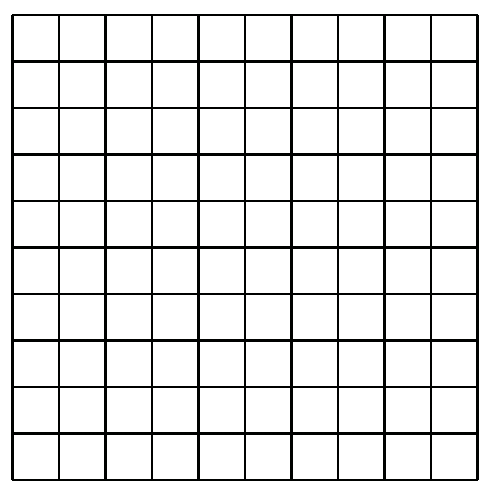
\includegraphics[width=4cm]{rect.png}
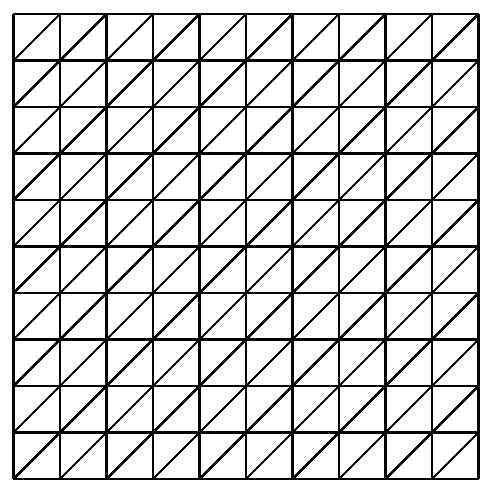
\includegraphics[width=4cm]{rect2.png}
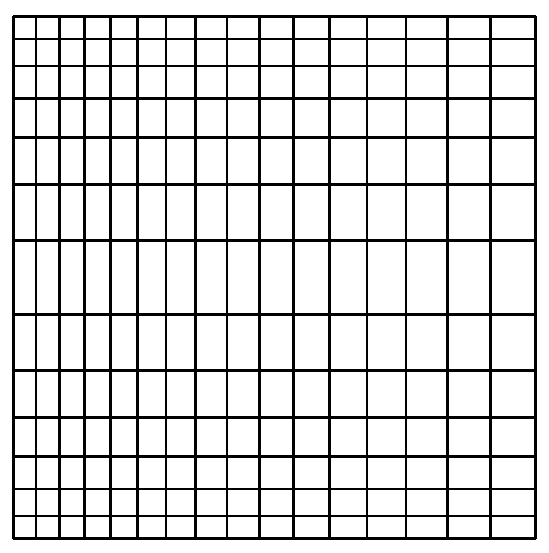
\includegraphics[width=4cm]{rect3.png}
\caption{Unit square with different meshes. a) 100 bilinear rectangles
b) 200 quadratic triangles c) 200 bilinear elements with nonuniform 
division.}
\label{fg:pic1}
\end{figure}

\subsection*{Tube: \texttt{tube.grd}}

The next case could be a simple 2D tube, as shown in Figure \ref{fg:pic2}a. 
Now the width is 5.0 which is reflected in 
the subcell boundaries. Again the mesh has some nonuniform division.

\verbatiminput{examples/tube.grd}
%
The variation of the case includes two mappings. The first mapping in Figure \ref{fg:pic2}b
maps the lower horizontal boundary so that it goes linearly between four points.
The second mapping in Figure \ref{fg:pic3}b sets the upper horizontal boundary 
to be a sinusoidal function with three periods.\\

\begin{verbatim}
Geometry Mappings 
! mode  line  limits(2)   Np  params(Np)
  1     0     1.0   1.0   8   0.0	0.1 1.0 -0.1 3.0 0.1 5.0 -0.1 
  5     1     1.0   1.0   4   0.0	5.0 3.0 -0.3
End 
\end{verbatim}
%
\begin{figure}[H]
\centering
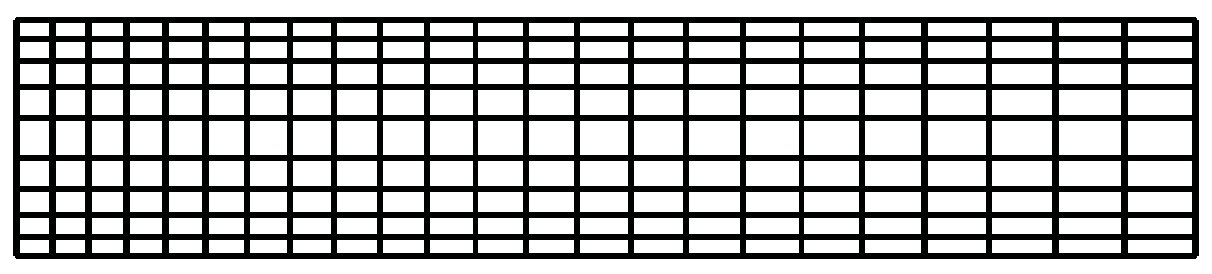
\includegraphics[width=8cm]{tube.png} 
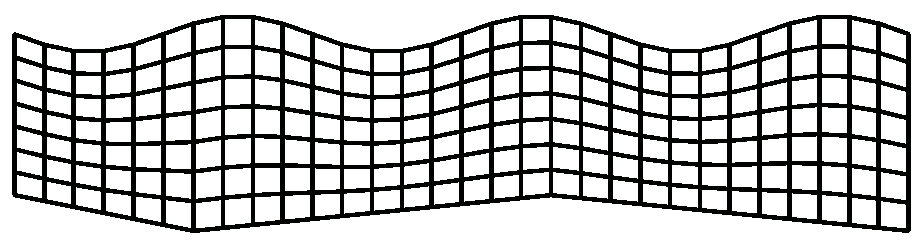
\includegraphics[width=8cm]{tube2.png}
\caption{Tube with 200 bilinear rectangles.
a) straight tube with 
two kinds of mesh refinement
b) sinusoidal and linear boundary mappings}
\label{fg:pic2}
\end{figure}

\subsection*{Square with holes: \texttt{holes.grd}}

The subcell structure may be quite complicated. This is reflected by an
example of a square with a large number of square holes, as shown in 
Figure \ref{fg:pic3}a. Even at such a complicated
case almost the desired amount of elements may be created quite quickly.
The second case in Figure \ref{fg:pic3}b with 81 holes and 112000 
elements was created in about a second an a normal PC.

\verbatiminput{examples/holes.grd}
%
\begin{figure}[H]
\centering
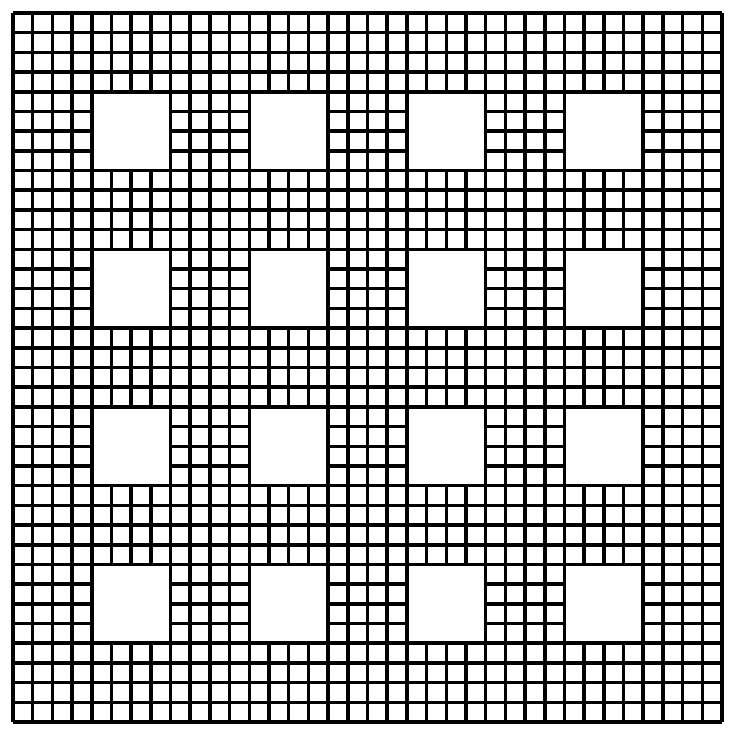
\includegraphics[width=5.5cm]{holes.png}
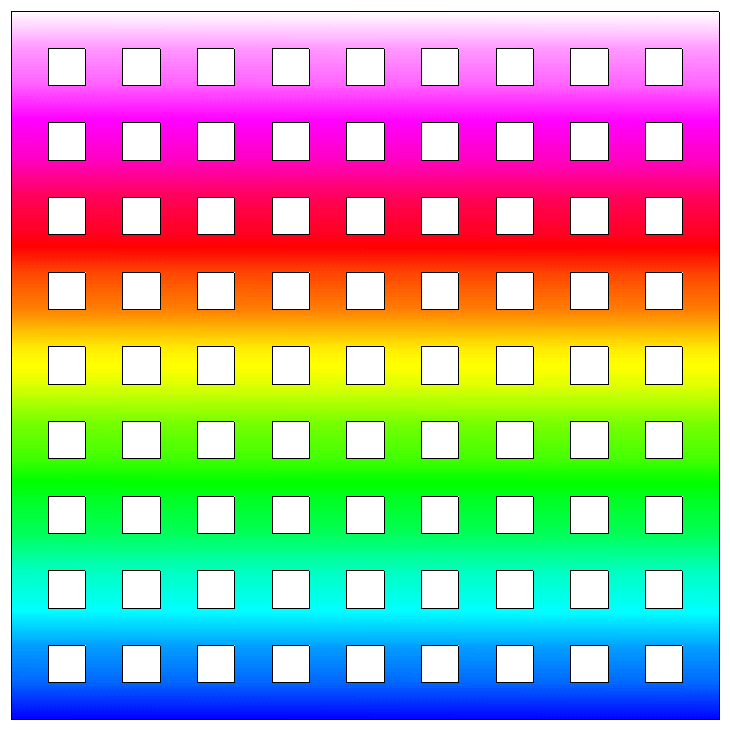
\includegraphics[width=5.5cm]{holes2.png}
\caption{Squares with holes: 
a) square with 16 square holes and 1040 elements,
b) square with 81 square holes and 112000 elements.}
\label{fg:pic3}
\end{figure}


\subsection*{Cross: \texttt{cross.grd}}

To show that multiple mappings may be used at the same time
a more complicated case is given. Here two horizontal and two vertical lines
are mapped, as shown in Figure \ref{fg:pic4}a. The mesher has the 
nice property that the same file may be used
to created multiple meshes with different settings. The other mesh in 
Figure \ref{fg:pic4}b is now the external mesh and it is divided to triangles.

\verbatiminput{examples/cross.grd}

\begin{figure}[H]
\centering
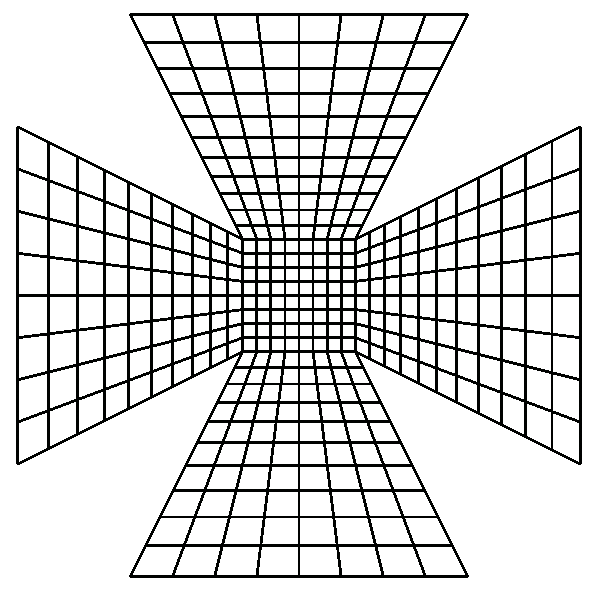
\includegraphics[width=5.5cm]{cross1.png}
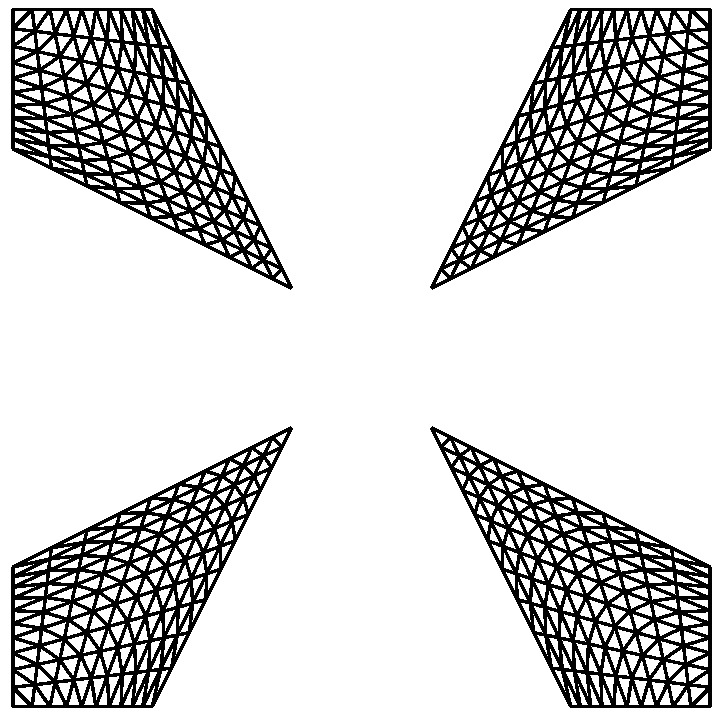
\includegraphics[width=5.5cm]{cross2.png}
\caption{Cross with shape used to create 2 computational meshes:
      a) the internal mesh of 400 bilinear rectangles
      b) the external mesh of 800 linear triangles.}
\label{fg:pic4}
\end{figure}

\subsection*{Hand-weight: \texttt{weight.grd}}

First we will create a 2D mesh, as shown in Figure \ref{fg:pic5}a.
Then we will use extrusion to create a 3D mesh, as shown in 
Figure \ref{fg:pic5}b.

\verbatiminput{examples/weight.grd}
%
The extrusion requires that there are subcells also in the 
$z$-direction. In this case only one subcell is set.
\begin{verbatim}
Coordinate System = Cartesian 3D
Subcell Divisions = 3 3 1
\end{verbatim}

\noindent
In addition all information that is given for $x$ and $y$
must now also be given for $z$. For example, the 
subcell boundaries in the extruded direction must be given.
\begin{verbatim}
Subcell Limits 3 = 0.0 0.5
\end{verbatim}

\begin{figure}[H]
\centering
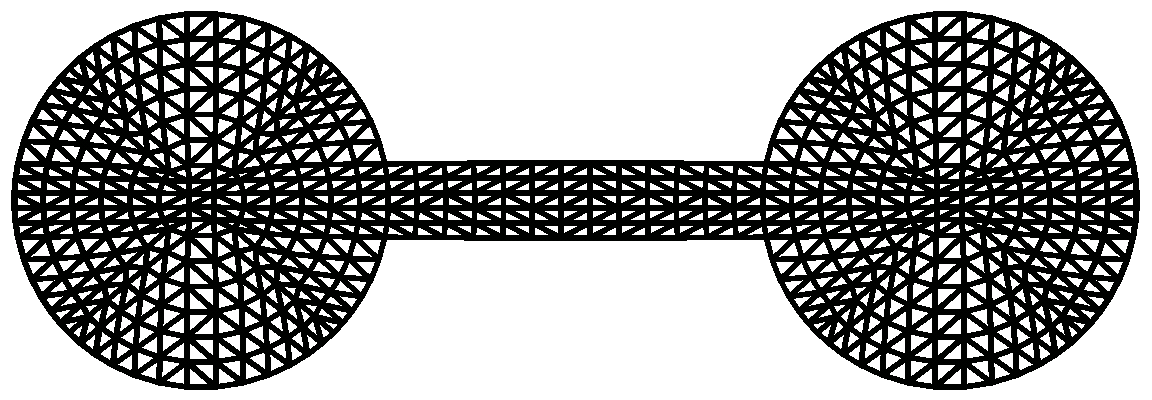
\includegraphics[width=8cm]{weight.png} 
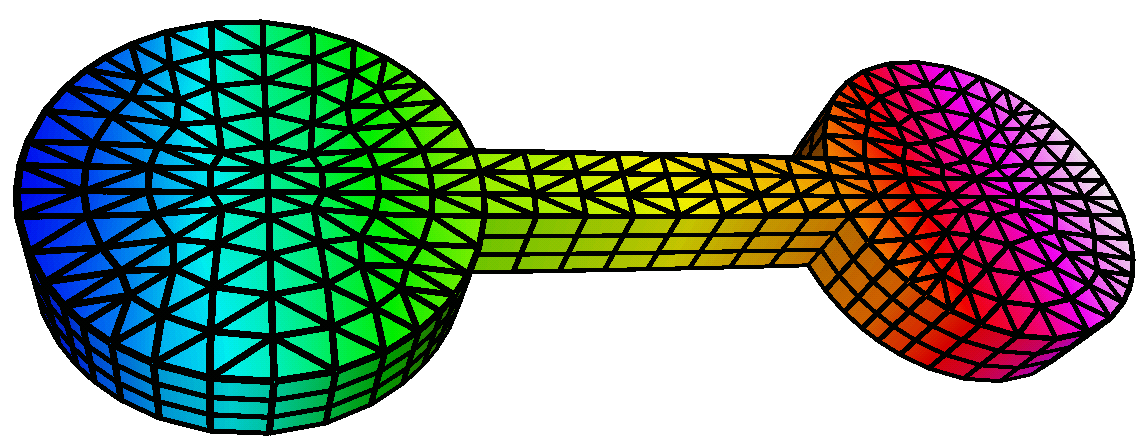
\includegraphics[width=8cm]{weight3.png}
\caption{Hand-weight consisting of two spheres and a joining tube
      a) 2D mesh with 1000 linear triangles
	b) extruded 3D mesh with 1200 prisms.}
\label{fg:pic5}
\end{figure}



\section{3D examples}

\subsection*{Shell of waves: \texttt{waves.grd}}

The originally 2D mesh may be given a third dimension with the help of mapping.
In this example two sinusoidal mappings are used. They have a amplitude
with different sign and therefore there is a phase-shift of 180 degrees between the 
two opposing sides, as shown in Figure \ref{fg:pic6}. 

\verbatiminput{examples/waves.grd}

\begin{figure}[H]
\centering
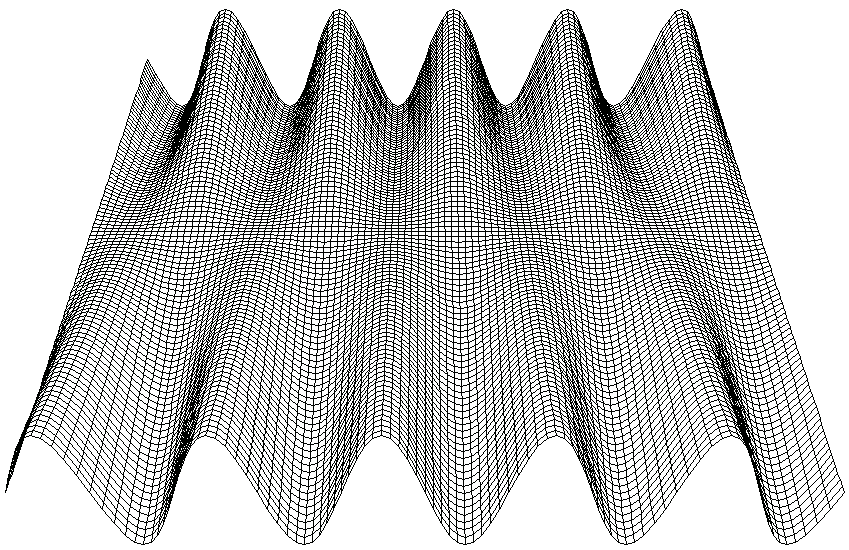
\includegraphics[width=7cm]{waves.png}
\caption{A shell with a wave pattern}
\label{fg:pic6}
\end{figure}


\subsection*{Shell consisting of two adjacent cones: \texttt{cones.grd}}

There are some cases where a mesh consisting of 2D elements 
may be used to model also 2D geometries. This is the case for
thin shells, for example. ElmerGrid does offer limited 
functionality for creating these. Only 
shells with rotational symmetry are possible to be created. 
Then the computational mesh is done for the $z$ and $\phi$ variables.
The missing radius must also be given.
After that $x=r \cos \phi$ and $y= r \sin \phi$.
Also limited possibilities to alter the radius as 
a function of positions is given. The same mappings may be used
as for 2D meshes in cartesian coordinates.

The examples shows a simple cylinder where a mapping is
used to create two cones, as shown in Figure \ref{fg:pic7}. 

\verbatiminput{examples/cones.grd}

\begin{figure}[H]
\centering
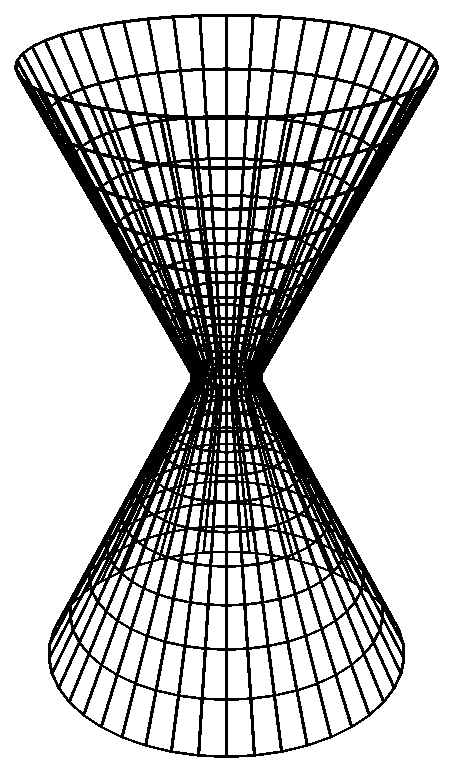
\includegraphics[width=6cm]{cones.png}
\caption{A 2D mesh mapped into two 3D cones}
\label{fg:pic7}
\end{figure}


\subsection*{A rolled shell: \texttt{cones.grd}}

The mappings out of plane may also be used to create a simple roll.
Now the angles extends to 3600 degrees making 10
full rotations. The radius goes linearly from 1 to 101 and thus the
roll has a spiraling structure, as shown in Figure \ref{fg:pic8}.

\verbatiminput{examples/roll.grd}

\begin{figure}[H]
\centering
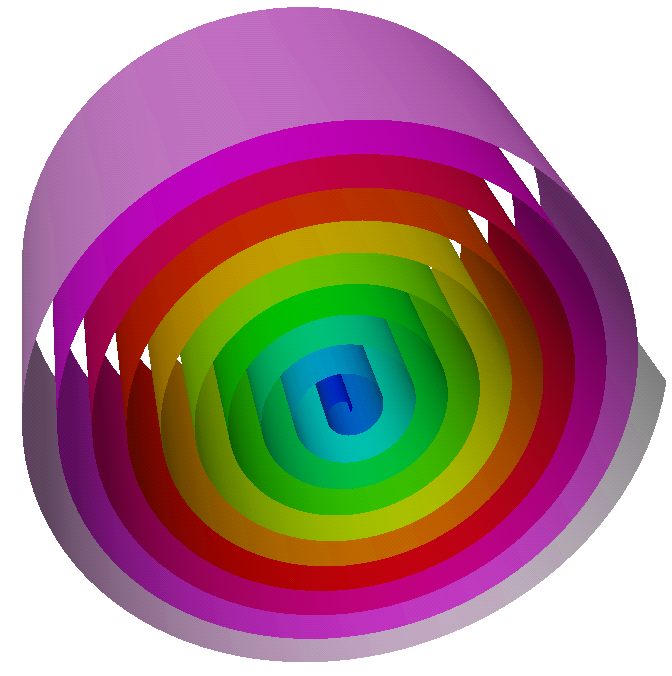
\includegraphics[width=7cm]{roll.png}
\caption{A rolled shell with a spiraling structure}
\label{fg:pic8}
\end{figure}


\subsection*{A hexagonal frame: \texttt{hexframe.grd}}

There is also a very special mapping for creating 
3D shell structures. The mapping is used to give an
angle for the shell. The angle is stepwise constant which makes
is possible to create polygonal 3D shells, as shown in Figure \ref{fg:pic9}.  

\verbatiminput{examples/hexframe.grd}

\begin{figure}[H]
\centering
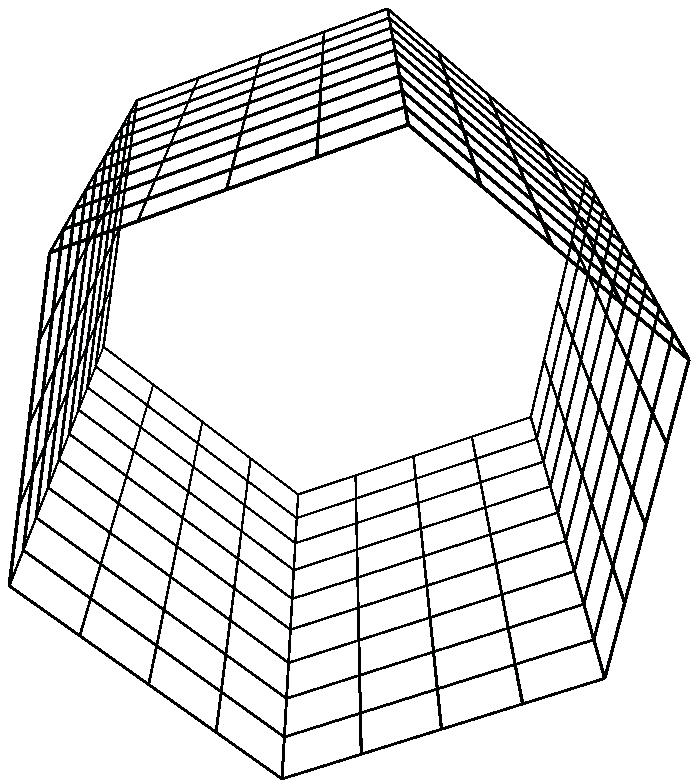
\includegraphics[width=7cm]{hexframe.png}
\caption{A hexagonal 3D frame made by mapping by angle}
\label{fg:pic9}
\end{figure}



\subsection*{Rotated step structure: \texttt{barrel.grd}}

Rotate a 2D step structure to create a 3D barrel shaped
structure, as shown in Figure \ref{fg:pic10}.

\verbatiminput{examples/barrel.grd}

\begin{figure}[H]
\centering
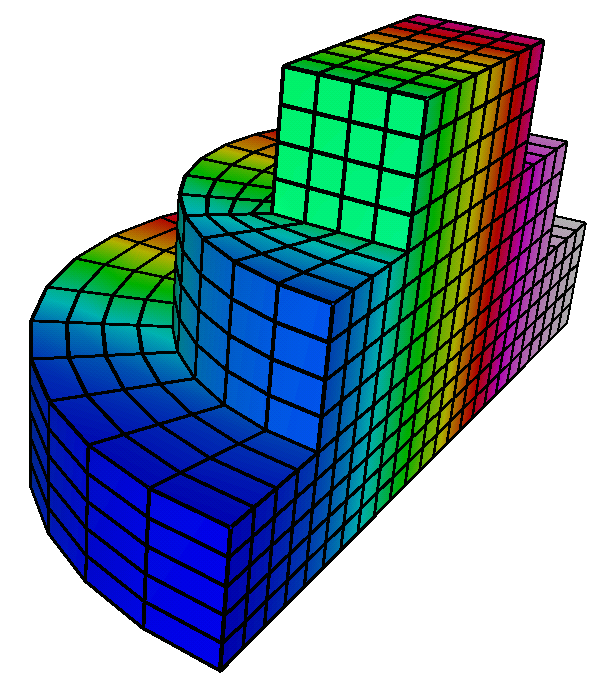
\includegraphics[width=8cm]{barrel.png}
\caption{Step structure rotated 180 degrees to create
      3D object with 1312 elements}
\label{fg:pic10}
\end{figure}


\subsection*{Extruded structure: \texttt{blocks.grd}}
The 2D structures may be extruded in the third dimension. 
Then the third dimension is added to the subcells
boundaries and to the mesh definitions, as shown in Figure \ref{fg:pic11}.

The material structure is always 2D. 
The given material structure may be 
extruded as is, or alternatively a selective extrusion for
different materials may be performed as is done in this example.
It is therefore possible to omit some materials, and to rename 
the extruded layer to some new material.

\verbatiminput{examples/blocks.grd}

\begin{figure}[H]
\centering
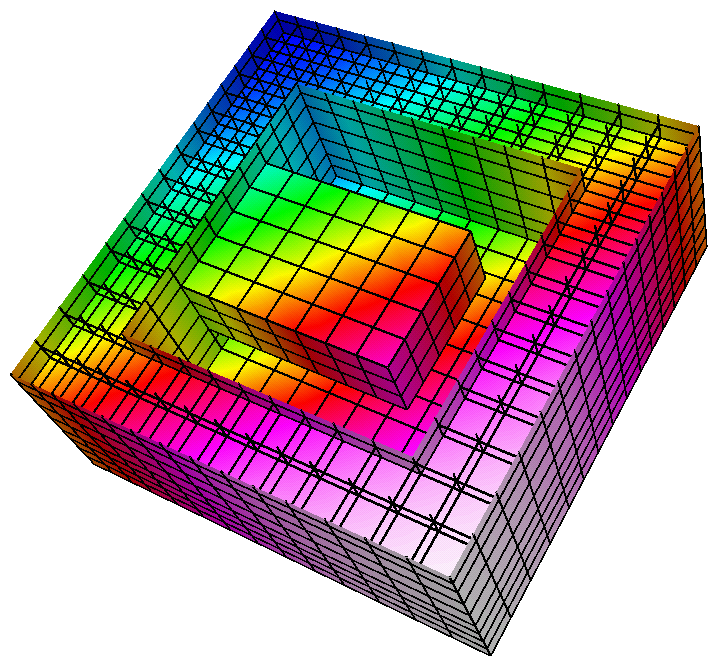
\includegraphics[width=8cm]{blocks.png}
\caption{Simple 3D structure created by selective extrusion. 
	The upper part has been removed for visualization purposes.}
\label{fg:pic11}
\end{figure}


\section{1D examples}

The ElmerGrid program was originally written for 2D mesh generation. 
However, it is also possible to make even more trivial one dimensional grids.
This is rarely needed as most FEM computations are at least two dimensions.

\subsection*{Line: \texttt{line.grd}}

The example of the 1D case is naturally a line segment -- there are no other kind of basic 1D structures.
It consists of two sections, the first one has a increasing mesh density to the right and the second one
has an even distribution of nodes, as shown in Figure \ref{fg:pic12}.
\verbatiminput{examples/line.grd}

\begin{figure}[H]
\centering
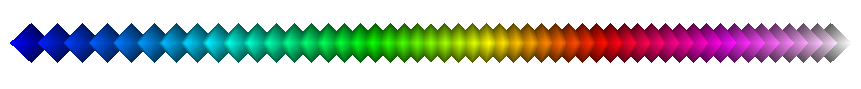
\includegraphics[width=12cm]{line.png} 
\caption{A line segment where the element nodes are marked with polygons.
The mesh has 50 elements and thus 51 nodes.}
\label{fg:pic12}
\end{figure}
